\chapter{Use cases}

\section{Factory Gate}

In the first use case, the control of the factory gate was implemented. In this use case, 2 buttons, 3 sensors, 2 actuators and 1 radio switch are used.

\begin{figure}[h]
    \centering
    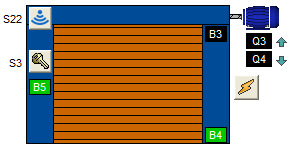
\includegraphics[width=0.70\textwidth]{images/usecase_factory_gate.png}
    \caption{Use Case Factory Gate}
    \label{fig:UseCaseFactoryGate}
\end{figure}

\begin{itemize}
    \item B3: Sensor that signals a fully opened gate.
    \item B4: Sensor that signals a fully closed gate.
    \item B5: Light sensor that is triggered when the gate is passed and leads to an immediate opening if the gate is about to be closed.    
    \item F2: Button with which the function of the light barrier B5 can be simulated.
    \item S3: Button used to control the opening and closing of the gate.
    \item S22: Radio switch that controls the opening and closing of the gate.
    \item Q3: Actuator that controls the gate motor and is used to open the gate.
    \item Q4: Actuator that controls the gate motor and is used to close the gate.
\end{itemize}

\section{Lifting Platform}

In this use case, the lifting platform of the factory has been simulated. The lifting platform is controlled by 3 buttons, which can be used to raise, lower or stop the platform. The end position of the platform is signaled by 2 sensors. The platform motor is controlled by 2 actuators. The overload protection of the motor can be tested using another button.

\begin{figure}[h]
    \centering
    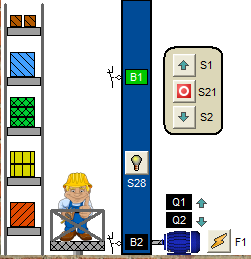
\includegraphics[width=0.55\textwidth]{images/usecase_lifting_platform.png}
    \caption{Use Case Lifting Platform}
    \label{fig:UseCaseLiftingPlatform}
\end{figure}

\begin{itemize}
    \item B1: Signals the top end position of the platform.
    \item B2: Signals the lowest end position of the platform.
    \item F1: Triggers the platform motor overload protection.
    \item S1: Signals the motor actuator to move the platform upwards.
    \item S2: Signals the motor actuator to move the platform downwards.
    \item S21: Stops the platform at its current position
    \item Q1: Activates the platform motor and moves the platform upwards.
    \item Q2: Activates the platform motor and moves the platform downwards.
\end{itemize}

\section{Hydraulic Press}

The hydraulic press is located on the first floor of the factory and is triggered by two buttons. If both buttons are activated at the same time, the press performs a downward movement. As soon as one of the two buttons is deactivated again, the press moves up again.

\begin{figure}[h]
    \centering
    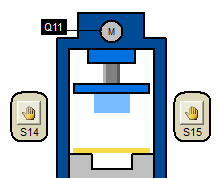
\includegraphics[width=0.55\textwidth]{images/usecase_hydraulic_press.png}
    \caption{Use Case Lifting Platform}
    \label{fig:UseCaseHydraulicPress}
\end{figure}

\begin{itemize}
    \item S14, S15: Buttons that must be activated to move the press down.    
    \item Q11: Motor that controls the movement of the press.
\end{itemize}

\section{Factory Light}

In the last use case, the control of the factory lighting was implemented. The factory hall is supplied with light via one lighting unit on each floor. The lights can be switched on or off using a total of 4 buttons.

\begin{figure}[h]
    \centering
    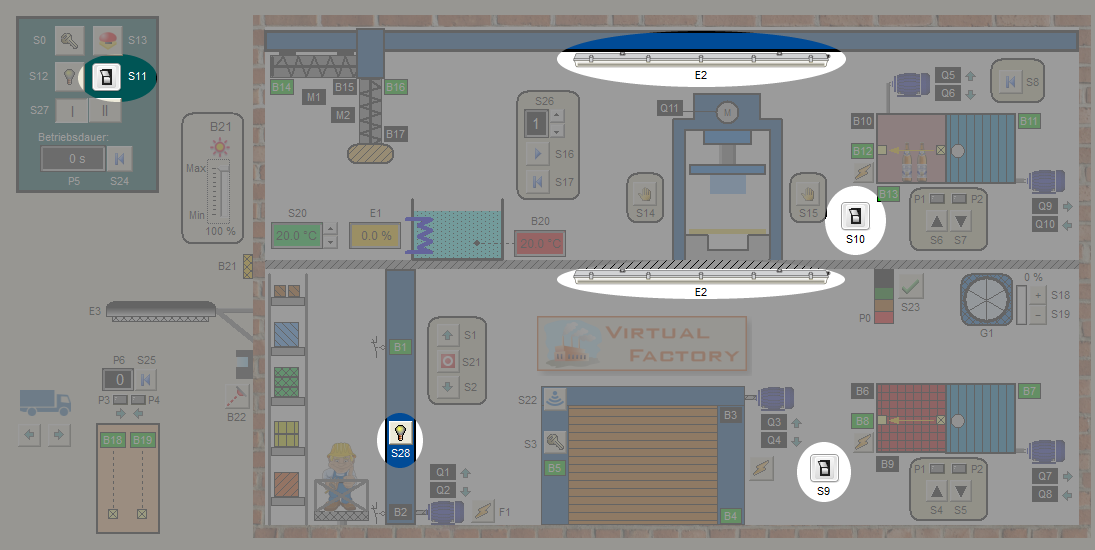
\includegraphics[width=0.80\textwidth]{images/usecase_factory_light.png}
    \caption{Use Case Lifting Platform}
    \label{fig:UseCaseFactoryLight}
\end{figure}

\begin{itemize}
    \item E2: Lights on the ground and first floor of the fabric hall.
    \item S9, S10, S11, S28: Button that must be activated or deactivate the hall light.
\end{itemize}

